\begin{figure}
	\centering
	\pgfplotsset{every axis legend/.append style={
		at={(1.05,0.5)},
		anchor=west}}
	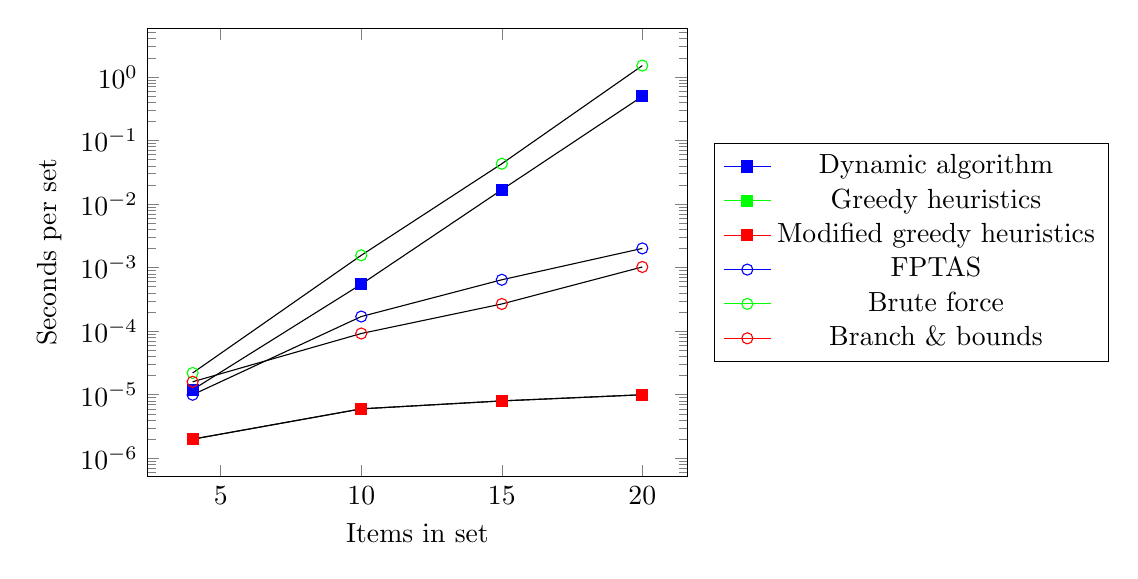
\begin{tikzpicture}
		\begin{semilogyaxis}[
			xlabel=Items in set,
			ylabel=Seconds per set,
			scatter/classes={
				solvePriceDynamic={mark=square*,blue},
				solveHungry={mark=square*,green},
				solveSingle={mark=square*,red},
				fptas={mark=o,blue},
				solveStupid={mark=o,green},
				solveSmart={mark=o,red}
				}
            ]
            
\addplot[scatter,scatter src=explicit symbolic]table[meta=label] {
x y label
4 .000012 solvePriceDynamic
10 .000548 solvePriceDynamic
15 .016784 solvePriceDynamic
20 .494500 solvePriceDynamic
};
\addplot[scatter,scatter src=explicit symbolic]table[meta=label] {
x y label
4 .000002 solveHungry
10 .000006 solveHungry
15 .000008 solveHungry
20 .000010 solveHungry
};
\addplot[scatter,scatter src=explicit symbolic]table[meta=label] {
x y label
4 .000002 solveSingle
10 .000006 solveSingle
15 .000008 solveSingle
20 .000010 solveSingle
};
\addplot[scatter,scatter src=explicit symbolic]table[meta=label] {
x y label
4 .000010 fptas
10 .000170 fptas
15 .000644 fptas
20 .002006 fptas
};
\addplot[scatter,scatter src=explicit symbolic]table[meta=label] {
x y label
4 .000022 solveStupid
10 .001562 solveStupid
15 .043078 solveStupid
20 1.507664 solveStupid
};
\addplot[scatter,scatter src=explicit symbolic]table[meta=label] {
x y label
4 .000016 solveSmart
10 .000092 solveSmart
15 .000268 solveSmart
20 .001024 solveSmart
};

			\addlegendentry{Dynamic algorithm}
			\addlegendentry{Greedy heuristics}
			\addlegendentry{Modified greedy heuristics}
			\addlegendentry{FPTAS}
			\addlegendentry{Brute force}
			\addlegendentry{Branch \& bounds}
		\end{semilogyaxis}
	\end{tikzpicture}
\caption{Average time per set with predominant light elements}
\label{plot:lightTime}
\end{figure}
